\documentclass[11pt,a4paper]{article}
\usepackage[T1]{fontenc}
\usepackage{lmodern,microtype,amsmath,amssymb,amsthm,mathtools,booktabs,array,xcolor}
\usepackage[top=22mm,bottom=24mm,left=26mm,right=26mm,headheight=14pt]{geometry}
\usepackage{fancyhdr,titlesec,tikz}
\definecolor{deep}{HTML}{173948}
\definecolor{teal}{HTML}{146C70}
\usepackage[colorlinks=true,linkcolor=deep,citecolor=teal,urlcolor=teal]{hyperref}
\usepackage{bookmark}
\numberwithin{equation}{section}
\newtheorem{theorem}{Theorem}[section]
\newtheorem{corollary}[theorem]{Corollary}
\newtheorem{proposition}[theorem]{Proposition}
\newtheorem{lemma}[theorem]{Lemma}
\titleformat{\section}{\Large\sffamily\bfseries\color{deep}}{\thesection}{.55em}{}
\titleformat{\subsection}{\large\sffamily\bfseries\color{deep}}{\thesubsection}{.55em}{}
\setlength{\emergencystretch}{2em}
\pagestyle{fancy}\fancyhf{}\lhead{\small\sffamily Hansen polytopes and prime-power supercongruences}
\rhead{\small\sffamily Research manuscript}\cfoot{\small\thepage}
\renewcommand{\headrulewidth}{.3pt}\raggedbottom
\hypersetup{pdftitle={Second minima of Mahler volume and flag count for unconditional reflexive polytopes},pdfsubject={Two predictions of Freij, Henze, Schmitt and Ziegler and conjectures of Guo and Schlosser}}
\begin{document}
\thispagestyle{plain}
\begin{center}
{\LARGE\bfseries\color{deep} Second minima of Mahler volume and flag count\par}
\vspace{2pt}
{\LARGE\bfseries\color{deep} for unconditional reflexive polytopes\par}\vspace{5pt}{\large Hansen polytope formulas and prime-power supercongruences\par}
\vspace{7pt}
{\small\sffamily Research manuscript \quad $\cdot$ \quad 20 November 2026}
\end{center}
\begin{abstract}
Freij, Henze, Schmitt and Ziegler computed the Mahler volume product and the number of complete flags for a family of Hansen polytopes through dimension ten. We prove both of their predicted formulas in every dimension by replacing a coordinate in a five-dimensional polytope with the norm of an arbitrary symmetric body. The volume multiplier follows from a section integral. The flag multiplier follows from the action of a reflection on face chains. We then expand the normalized volume product of an arbitrary split-graph Hansen polytope as a positive sum over configurations of permutation cycles. The positive expansion gives the second and third distinct volume products in the split-graph Hansen class. Coordinate-section inequalities extend the second-value result to all unconditional reflexive lattice polytopes. In every dimension $d\ge4$ the second normalized values of Mahler volume and flag count are respectively $1+(d-4)!/d!$ and $1+4(d-4)!/d!$. They are attained by precisely the same polytopes. As a consequence, the smallest positive defect in Sidorenko\textquoteright s linear-extension inequality is $(d-4)!$.

A second application concerns the even-power hypergeometric sums of Guo and Schlosser. A quadratic finite difference and a double zero in a $p$-adic parameter give their Conjectures 2 and 3 at every prime-power height. The predicted exponents are both sharp at every height for $p=5$. A calculation at roots of unity proves their Conjectures 4 and 6 in conjunction with their later fourth-power theorem. A modular counterexample disproves their Conjecture 7.
\end{abstract}
\section*{The original questions}
For a $d$-polytope $P$ containing the origin, write $P^\circ$ for its polar. A reflexive lattice polytope has interior origin and lattice polar. Unconditionality means invariance under the independent sign changes of all coordinates. Normalized Mahler volume is $d!|P||P^\circ|/4^d$, and normalized flag count is $\mathrm{ff}(P)/(2^d d!)$. Each has minimum one on this class. Theorem~\ref{thm:both} determines the next distinct value and all its equality graphs.\par\medskip The first part addresses the two formulas printed in Section 5 of the 2013 paper of Freij, Henze, Schmitt and Ziegler~\cite{FHSZ}. They concern the particular Hansen polytopes built in their Corollary 19. One can read the two predictions as a question about why different threshold graphs give exactly the same two answers. Theorem~\ref{thm:hansen-lift} explains this independence before the threshold assumption is made. Winter's general inequality compares the two quantities~\cite{Winter}. The exact excesses found here have a ratio of four after the Hanner normalizations.
 
The second part addresses the published numbering in Section 5 of Guo and Schlosser's \emph{Even powers} paper~\cite{GS}. The changing hypergeometric parameters make the sum at one prime-power height quite different from the sum at the next. Keeping the summation length fixed and varying a separate parameter exposes the second-order vanishing responsible for the stronger of the two classical congruences.

Two methodological starting points in the supplied corpus are the composition of counts conditioned on a fibre in entry 041 and the separation of terminating identities from lifting steps in entry 214, round 18~\cite{Corpus}. Below, the convex fibres, the action on chains, the auxiliary arithmetic family, and the two orders of vanishing are all derived explicitly.

\begin{center}\small
\begin{tabular}{c@{\quad}r@{\quad}r@{\quad}r}
\toprule
Dimension & Minimum flag count & Second flag count & Second normalized volume product\\
\midrule
4 & 384 & 448 & $25/24$\\
5 & 3,840 & 3,968 & $121/120$\\
6 & 46,080 & 46,592 & $361/360$\\
\bottomrule
\end{tabular}
\end{center}
\clearpage

\section{The two Freij--Henze--Schmitt--Ziegler predictions}
\label{sec:hansen-volume}
For an origin-symmetric convex body $Q$ of dimension $t$ with the origin in its interior, write
\[
 m(Q)=\frac{t!}{4^t}|Q|\,|Q^\circ|,\qquad
 h(Q)=\frac{\mathrm{ff}(Q)}{2^t t!}
\]
where $Q^\circ=\{v:\langle v,y\rangle\le1\text{ for all }y\in Q\}$ and $\|y\|_Q=\inf\{\lambda>0:y\in\lambda Q\}$. Here $h$ is used only for polytopes, and $\mathrm{ff}$ counts maximal chains of faces. Define a body of dimension $d=t+4$ by
\begin{equation}
 \mathcal H(Q)=\left\{(a,b,c,e,y):\ |a|+|b|\le1,\quad
 |b|+|c|+\|y\|_Q\le1,\quad |c|+|e|\le1\right\}.
 \label{eq:calH-def}
\end{equation}
\begin{theorem}\label{thm:hansen-lift}
For every $t\ge1$ and every $Q$ as above,
\[
 m(\mathcal H(Q))=m(Q)\left(1+\frac{t!}{(t+4)!}\right).
\]
When $Q$ is polytopal, one also has
\[
 h(\mathcal H(Q))=h(Q)\left(1+4\frac{t!}{(t+4)!}\right).
\]
\end{theorem}

For a graph $G$ on $n$ vertices let $Q(G)$ be the convex hull of incidence vectors of its stable sets. Write $H(G)=\operatorname{conv}((1,Q(G))\cup(-1,-Q(G)))$. If $a,b,c,e$ form a path in this order, the notation $P_4\times T$ used in~\cite{FHSZ} attaches a threshold graph $T$ by joining both middle vertices $b,c$ to every vertex of $T$. The authors reported the following two expressions through dimension ten and explicitly predicted them in every dimension.
\begin{corollary}\label{thm:hansen-flags}
For every threshold graph $T$ on $m\ge0$ vertices, $d=m+5$ and $P=H(P_4\times T)$,
\[
 |P|\,|P^\circ|=\frac{4^d}{d!}\left(1+\frac{(d-4)!}{d!}\right),\qquad
 \mathrm{ff}(P)=2^d\big(d!+4(d-4)!\big).
\]
\end{corollary}

\subsection{The polar and its sections}
Put $K=\mathcal H([-1,1])$ and denote its last coordinate by $z$. For any convex $K$ invariant under changing the sign of $z$ define $K(Q)=\{(x,y):(x,\|y\|_Q)\in K\}$. Write $h_C(u)=\sup_{v\in C}u\cdot v$. Maximizing over $y\in zQ$ gives
\[
 h_{K(Q)}(u,v)=h_K\big(u,h_Q(v)\big),\qquad
 K(Q)^\circ=K^\circ(Q^\circ).
\]
The defining inequalities for $K$ show that its polar is the convex hull of signed incidence vectors on $ab,bcz,ce$, where each coordinate sign varies independently. The vertices of $K$ are the signed incidence vectors on $aez,ac,be$. One can see this by taking one orthant: for $b,c,z\ge0$ with $b+c+z\le1$, the two remaining nonnegative coordinates range independently over $[0,1-b]$ and $[0,1-c]$. This section is generated by the boxes above the vertices of the simplex in $(b,c,z)$, as their two side lengths are affine there. Taking all sign choices, the supports not on the three displayed lists are contained in one of them. Thus $K$ and its polar are related by the permutation $a\mapsto b,\ e\mapsto c,\ b\mapsto e,\ c\mapsto a$, which fixes $z$.

Let $S(z)$ denote the four-dimensional section-volume at $0\le z\le1$. Orthant integration gives
\[
 S(z)=16\int_{s,u\ge0,\ s+u\le1-z}(1-s)(1-u)\,ds\,du
 =16\left(\frac{(1-z)^2}{2}-\frac{(1-z)^3}{3}+\frac{(1-z)^4}{24}\right).
\]
Since $|\{y:\|y\|_Q\le z\}|=z^t|Q|$, integration and the beta integral yield
\[
 \frac{|K(Q)|}{|Q|}=t\int_0^1z^{t-1}S(z)\,dz
 =16\frac{t!}{(t+4)!}(t^2+5t+5).
\]
The same multiplier applies to the polar. The identity $(t^2+5t+5)^2=(t+1)(t+2)(t+3)(t+4)+1$ proves the volume assertion of Theorem~\ref{thm:hansen-lift}.

\subsection{Replacing a coordinate by a norm}
Let $K\subset\mathbb R^{p-1}\times\mathbb R$ be a full-dimensional polytope invariant under $\sigma(x,z)=(x,-z)$, containing zero in its interior. For an origin-symmetric $t$-dimensional polytope $Q$ with norm $\|\cdot\|_Q$, define
\[
 K(Q)=\{(x,y):(x,\|y\|_Q)\in K\}.
\]
For $j\ge1$ let $N_j(K)$ be the number of full flags of $K$ containing exactly $j$ faces moved by $\sigma$. Then
\begin{equation}
 \frac{\mathrm{ff}(K(Q))}{\mathrm{ff}(Q)}
 =\frac12\sum_{j=1}^{p} N_j(K)\binom{t+j-2}{j-1}.
 \label{eq:hansen-flag-sub}
\end{equation}
Here $t=1$ is allowed.

To prove the formula, classify each nonempty face of $K$ into three types: $A$ if contained in $z=0$, $B$ if invariant under $\sigma$ and meeting $z>0$, and $C$ if moved by $\sigma$. A type $C$ face lies in one of the two closed halfspaces with some point off $z=0$: a supporting functional with nonzero last coefficient has this property, and a functional with zero last coefficient exposes an invariant face. Choose the upper representative of each type $C$ pair. The faces of $K(Q)$ have the following description.
\[
\begin{array}{c|l|c}
\text{base data}&\text{lifted face}&\text{dimension}\\\hline
 A &(x,0),\quad(x,0)\in A &\dim A\\
 B &(x,zu),\quad (x,z)\in B,\ z\ge0,\ u\in Q &\dim B+t-1\\
 (C,E)&(x,zu),\quad (x,z)\in C,\ u\in E &\dim C+\dim E
\end{array}
\]
Here $E$ is a nonempty proper face of $Q$. Indeed, maximize a functional $(w,v)$, first on each fibre $zQ$. The maximum there is $zh_Q(v)$, where $h_Q(v)=\max_{u\in Q} v\cdot u$. With $v=0$ this gives an invariant base face. With $v\ne0$ it gives an upper base face, and the maximizing fibre is $zE(v)$. Conversely an upper supporting slope can be realized by scaling a normal to any chosen $E$. Every invariant face admits an exposing functional with last coefficient zero, by averaging that functional with its reflection. The three rows are distinct, and $C,E$ are recovered from the lifted face by $(x,y)\mapsto(x,\|y\|_Q)$ and its fibre at positive height. The dimension in the last row follows because a supporting hyperplane of $E$ avoids the origin: on its cone the height $z$ is a linear functional of $y$, leaving $\dim E$ independent fibre coordinates. For row $B$ the projection onto $x$ has dimension $\dim B-1$, and its fibre above a point with positive height has dimension $t$.

On a lifted flag the three types can occur only in order $A,C,B$, allowing empty initial and final proper-face segments and counting the whole polytope as type $B$. Within type $C$ inclusion is equivalent to inclusion in both base and fibre. At a transition $A\to C$ a cover must start with $E$ a vertex, and at $C\to B$ it must finish with $E$ a facet, by the displayed dimensions. The same vertex conclusion holds when the first nonempty face is already type $C$. A direct $A\to B$ cover is impossible for $t\ge2$. In the base $t=1$, an entire full flag of invariant faces is also impossible: their barycentres would all lie in $z=0$, whereas the barycentres of any full flag, including the whole polytope, are affinely independent. In any lifted flag compress repeated base faces. The resulting base chain is saturated by the dimension formulas, starts at a vertex, and chooses the upper member throughout the type $C$ segment. Each base flag with $j$ type $C$ faces contributes $\mathrm{ff}(Q)$ full fibre flags, and the $t-1$ fibre steps interleave with $j-1$ base steps in $\binom{t+j-2}{j-1}$ ways. Reflection pairs the upper and lower base chains without fixed chains. This proves~\eqref{eq:hansen-flag-sub}.

\subsection{Full flags of the five-dimensional core}
The signed vertex and facet descriptions of $K$ above each have sixteen members. A verification program appears at the end of the manuscript. Equivalently their supports are the maximal stable sets and maximal cliques, respectively, of the graph $J_0$ on $a,b,c,e,z$ with edges $ab,bc,ce,bz,cz$. Reflecting coordinate $z$, the full-flag counts are
\[
 (N_1,N_2,N_3,N_4,N_5)=(896,768,768,768,768).
\]
Here is a finite reproducible enumeration entirely in sets of at most sixteen vertices. Take $V$ and $W$ to be all signed incidence vectors of the three stable sets and three cliques, respectively. Start with $\mathcal F=\{V\}$. For each $w\in W$ replace $\mathcal F$ by its union with $\{F\cap\{v\in V:w\cdot v=1\}:F\in\mathcal F\}$. This enumerates all faces by their vertex sets, including the empty set. For the following recurrence process the $260$ resulting subsets by increasing cardinality. Set $r(\varnothing)=-1$, $D(\varnothing)=1$. For nonempty $F$ use
\[
 r(F)=1+\max_{H\in\mathcal F,\ H\subsetneq F}r(H),\qquad
 D(F)=X^{\mathbf1_{\sigma F\ne F}}
 \sum_{\substack{H\in\mathcal F,\ H\subsetneq F\\r(H)=r(F)-1}} D(H).
\]
The recurrence counts saturated chains by their number of moved faces, giving $D(V)=896X+768(X^2+X^3+X^4+X^5)$. Substitution in~\eqref{eq:hansen-flag-sub} and the hockey-stick identity give
\[
 \frac{\mathrm{ff}(K(Q))}{\mathrm{ff}(Q)}
   =64+384\binom{t+4}{4}.
\]
This proves the flag assertion of Theorem~\ref{thm:hansen-lift} for every $t$-dimensional origin-symmetric polytope $Q$.

\subsection{Recovering the original Hansen polytope}
For a perfect graph $J$ write $U(J)=\{x:(|x_i|)_i\in Q(J)\}$. Its inequalities are $\sum_{i\in D}|x_i|\le1$ over maximal cliques $D$, and its vertices are the signed incidence vectors of the maximal stable sets. The clique description is the stable-set-polytope theorem for perfect graphs. For the split graphs used here it has a direct proof. Given nonnegative coordinates satisfying all clique inequalities, choose at most one clique-part vertex $i$ with probability $x_i$, leaving the remaining mass for an empty choice. A stable-part vertex $j$ is available with probability $1-\sum_{i\sim j}x_i\ge x_j$, with the sum over the clique part. Include it on the available event with conditional probability equal to $x_j$ divided by this availability, and omit it when the availability is zero. This realizes all coordinates as the means of incidence indicators of one stable set. Taking convex hulls of all coordinate sign choices gives the signed vertex description. A smaller support belongs to the convex hull of the sign choices on a maximal support. A signed maximal support is exposed by the signed sum of its own coordinates.
For a split graph $G=C\cup S$, adjoin a new vertex $o$ adjacent to every member of $C$ and none of $S$, and call the graph obtained $J$. Then $H(G)$ is linearly equivalent to $U(J)$. Indeed make the invertible linear change from $(s,x_C,x_S)$ to
\[
 z_o=s-\sum_{c\in C}x_c,\qquad z_c=x_c,\qquad
 y_j=2x_j-s+\sum_{c\sim j,\,c\in C}x_c\quad(j\in S).
\]
On a Hansen vertex $\pm(1,\mathbf1_A)$ the coordinates $z$ give a signed unit vector, labelled $o$ if $A\cap C=\varnothing$, and otherwise labelled by its unique clique vertex $c$. For label $i$ the $y_j$ run independently over $\{-1,1\}$ for $j\in S\setminus N_J(i)$ and are zero on the other coordinates. These are precisely the signed maximal stable sets of $J$.

Now take $G=P_4\times T$, splitting $T$ into its dominating and isolated insertion vertices in a threshold construction. The graph induced on $T$ and $o$ in $J$ is the threshold graph $T'$ obtained by starting with $o$ and making those same insertions. Both $b,c$ are joined to the whole block $T'$, and neither $a$ nor $e$ is joined to it. Thus $J$ is obtained from the fixed five-vertex graph $J_0$ with edges $ab,bc,ce,bo,co$ by substituting $T'$ for $o$. The clique inequalities give
\[
 U(J)=K(Q),\qquad K=U(J_0),\quad Q=U(T'),\quad t=m+1.
\]
In fact a clique through $o$ has its $o$-term replaced by the maximum of the clique sums in $T'$, which is exactly $\|y\|_Q$. At an isolated insertion $U(T')$ takes a Cartesian product with a segment, and at a dominating insertion it takes a direct sum with a segment. A Cartesian product of a $k$-polytope with a segment has $2(k+1)$ times as many full flags, by interleaving the segment step in a pair of flags. The same is true for direct sums by polarity. For a Cartesian product with a segment the volume product is multiplied by $4/(k+1)$, since its polar is a bipyramid, and the same holds under the dual operation. Hence $m(Q)=h(Q)=1$. Theorem~\ref{thm:hansen-lift} now implies Corollary~\ref{thm:hansen-flags}.


\subsection{The full face vector}
The face classification also yields all face numbers of the substituted polytope. Let $f_Q(u)=\sum_{i=0}^{t} f_i(Q)u^i$ include the whole polytope and omit the empty face. In the order of increasing dimension, the three rows of the classification for the five-dimensional core give the following counts. Type $C$ uses only the upper representative in each pair.
\[
\begin{array}{c|rrrrrr}
\dim&0&1&2&3&4&5\\\midrule
 A&8&20&16&4&0&0\\
 B&0&4&16&20&8&1\\
 C&4&20&33&20&4&0
\end{array}
\]
If $A(u),B(u),C(u)$ are the polynomials with these coefficients, the dimensions in the classification give
\[
 f_{K(Q)}(u)=A(u)+u^{t-1}B(u)+C(u)\big(f_Q(u)-u^t\big).
\]
This gives a check directly against the original article. For a threshold block, $f_Q(1)=3^t$, since taking a product with a segment triples the number of nonempty faces and polarity preserves that count. As $A(1)=48$, $B(1)=49$, $C(1)=81$, the formula gives $3^{t+4}+16$, the already proved Corollary 19 of~\cite{FHSZ}. For the five-dimensional case the two new formulas instead give $\mathrm{ff}=3968$ and volume product $1936/225$.

\section{The sharp second minimum for split graphs}\label{sec:split-correction}
Write a split graph as a clique $C$ and a stable set $S$, with $c=|C|$, $s=|S|$ and $h=c+s$. Let $A$ be its bipartite adjacency matrix. Applying the split-graph change of coordinates from Section~\ref{sec:hansen-volume} and replacing its distinguished coordinate by $\|y\|_Q$ gives the following inequalities. In particular $K_A([-1,1])$ below is linearly equivalent to $H(G)$. For a threshold extension $G\times T$, the inserted vertices are joined to every vertex of $C$ and none of $S$. The same argument as for $P_4$ replaces the distinguished coordinate by the threshold body of dimension $|T|+1$. In these coordinates the inequalities are
\[
 \sum_{i\in C}|x_i|+\|y\|_Q\le1,\qquad
 |w_j|+\sum_{i\in N(j)}|x_i|\le1\quad(j\in S).
\]
Denote the resulting body by $K_A(Q)$ and put $u=t+1$, where $t=\dim Q$. Let $p_4(A)$ count the induced four-vertex paths in the split graph, equivalently the $2\times2$ submatrices of $A$ equal to a permutation matrix. We claim that for each fixed $A$,
\begin{equation}
 \frac{m(K_A(Q))}{m(Q)}=1+\frac{p_4(A)}{t^4}+O_A(t^{-5}).
 \label{eq:p4-asym}
\end{equation}
The error constant is independent of $Q$.

For a cycle $B$ on a subset of $S$, write $n_0(B)=|\{i\in C:A_{ij}=0\text{ for all }j\in B\}|$. Define
\[
 A_*(u)=\sum_{\pi\in\mathrm{Sym}(S)}\prod_{B\in\mathrm{cyc}(\pi)}(u+n_0(B)),\qquad
 B_*(u)=(\mathbf1-A^{\mathsf T})_*(u).
\]
Here the second expression applies the same definition with the two parts exchanged and the bipartite entries complemented. Then
\begin{equation}
 \frac{m(K_A(Q))}{m(Q)}=\frac{A_*(u)B_*(u)}{(u)_{h}},\qquad (u)_j=u(u+1)\cdots(u+j-1).
 \label{eq:hansen-cycle-formula}
\end{equation}
For a derivation, after orthant integration in the $w_j$ and integration over $y$ the remaining integral is proportional to
\[
 \int_{x_i\ge0,\,\sum x_i\le1}
 (1-\textstyle\sum x_i)^t\prod_{j\in S}\left(1-\sum_{i\in N(j)}x_i\right)\,dx.
\]
More precisely $|K_A(Q)|/|Q|$ is $2^{h}t!/(t+c)!$ times the expectation of $\prod_{j\in S}(1-\sum_{i\in N(j)}X_i)$ over the Dirichlet vector $(X_0,(X_i)_{i\in C})$ with parameters $(u,1,\ldots,1)$ and $X_0=1-\sum X_i$. A factor is $X_0+\sum_{i:A_{ij}=0}X_i$. Expand the product by assigning its $s$ labels to admissible categories. The Dirichlet moment numerator for $k$ labels in a category of parameter $v$ is $(v)_k=\sum_{\sigma\in\mathrm{Sym}(k)} v^{\#\mathrm{cyc}(\sigma)}$, and its common denominator is $(u+c)_s$. Thus every cycle of the resulting permutation chooses either category zero with weight $u$ or a common nonneighbor with weight one. Consequently $|K_A(Q)|/|Q|=2^h t! A_*(u)/(t+h)!$. The polar uses the complemented transpose matrix and $Q^\circ$: its signed supporting vectors correspond to cliques, and those of the polar to stable sets. Equivalently, polarize the one-coordinate core before replacing its coordinate, as in the support-function formula. Applying the same volume computation gives~\eqref{eq:hansen-cycle-formula}.

\subsection{Cycles of the two permutations}
In the product $A_*(u)B_*(u)$ choose a permutation of each colour class. Every monochrome cycle either has no outgoing arrow, carrying weight $u$, or sends an arrow to a chosen vertex in an opposite-colour cycle. A cycle on $S$ can point to a common nonneighbor and a cycle on $C$ to a common neighbor. Consider the weakly connected components of this directed graph on cycles. Each component is either rooted, with exactly one unanchored cycle, or contains a directed cycle and has no root. On a nonempty set $W$ of original vertex labels let $T(W)$ and $U(W)$ count connected rooted and rootless configurations, respectively. Disjoint assembly gives
\begin{equation}
 A_*(u)B_*(u)=\sum_{\mathcal P\,\vdash\, C\cup S}
 \prod_{W\in\mathcal P}\bigl(uT(W)+U(W)\bigr).
 \label{eq:hansen-components}
\end{equation}
In comparison, $(u)_h=\sum_{\mathcal P}\prod_{W\in\mathcal P}u(|W|-1)!$ by the cycle decomposition of permutations. 

No directed cycle of length two is possible: the two target vertices would need to be both adjacent and nonadjacent. A rootless component therefore contains at least four labels. With exactly four it must consist of singleton cycles around a directed four-cycle. This occurs precisely on a two-by-two permutation submatrix, with exactly one choice of arrows. Thus $U(W)$ for $|W|\le4$ is its induced-$P_4$ indicator.

\begin{center}
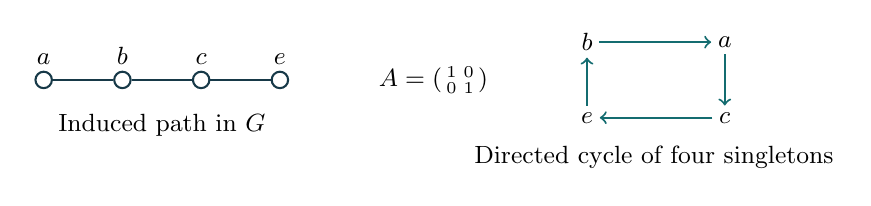
\begin{tikzpicture}[x=1cm,y=1cm,every node/.style={font=\small},line width=.75pt]
\foreach \name/\px/\py in {a/0/0,b/1/0,c/2/0,e/3/0}{
  \node[circle,fill=white,draw=deep,inner sep=2.1pt] (\name) at (\px,\py) {};
  \node[above=2pt] at (\name) {$\name$};
}
\draw[deep] (a)--(b)--(c)--(e);
\node at (1.5,-.57) {Induced path in $G$};
\node at (4.95,0) {$A=\left(\begin{smallmatrix}1&0\\0&1\end{smallmatrix}\right)$};
\foreach \name/\letter/\px/\py in {p/b/6.9/.48,q/a/8.65/.48,r/c/8.65/-.48,v/e/6.9/-.48}
   \node[inner sep=2.1pt] (\name) at (\px,\py) {$\letter$};
\draw[->,teal] (p)--(q);\draw[->,teal] (q)--(r);
\draw[->,teal] (r)--(v);\draw[->,teal] (v)--(p);
\node at (7.75,-.98) {Directed cycle of four singletons};
\end{tikzpicture}
\end{center}
\subsection{The exact number of rooted configurations}
We show that $T(W)=(|W|-1)!$ for every nonempty $W$. Orient the complete bipartite graph on $C,S$ by placing $j\to i$ for $j\in S,i\in C$ when $A_{ij}=0$, and $i\to j$ otherwise. In this orientation a monochrome cycle may attach to a vertex exactly when each of its labels points to that vertex. Carry out formal series operations over
\[
 \mathcal R=\mathbb Q[x_i:i\in C\cup S]/(x_i^2:i\in C\cup S).
\]
The coefficient of $x_W=\prod_{i\in W}x_i$ records objects whose distinct labels are exactly $W$. This quotient removes products whose label sets overlap.

A decorated vertex consists of a vertex $i$ and all the directed branches entering that vertex. Let its enumerator be $Y_i$. Each incoming branch begins with a cyclically ordered nonempty list of decorated vertices, whose underlying labels $j$ obey $j\to i$. These incoming cycles form an unordered set. For disjointly labelled objects of enumerator $L$, nonempty cycles have enumerator $\sum_{k\ge1}L^k/k$, since a cyclic ordering has $k$ linear representatives. Unordered sets have enumerator $\exp$, by the corresponding $k!$ factor. Thus the defining recursion on the number of labels is
\[
 Y_i=x_i\exp\!\left(\sum_{k\ge1}\frac{(\sum_{j\to i}Y_j)^k}{k}\right)
     =\frac{x_i}{1-\sum_{j\to i}Y_j}.
\]
Every connected rooted configuration has one root cycle, which is a monochrome nonempty cycle of decorated vertices. Consequently its enumerator is
\[
 \mathcal T=-\log(1-Y_C)-\log(1-Y_S),
 \qquad Y_C=\sum_{i\in C}Y_i,\quad Y_S=\sum_{j\in S}Y_j .
\]
Summing the defining identities $x_i=Y_i(1-\sum_{j\to i}Y_j)$ counts each product $Y_iY_j$ for a cross pair exactly once. Hence
\[
 \sum_i x_i=Y_C+Y_S-Y_CY_S,
 \qquad \mathcal T=-\log(1-\textstyle\sum_i x_i).
\]
The coefficient of $x_W$ on the right is $(|W|-1)!$, proving the assertion. Notice that all logarithms and exponentials here are finite sums on nilpotent arguments.

Let $D(W)$ count configurations on $W$ all of whose components are rootless, and set $D(\varnothing)=1$. On the complement of $W$, all components are rooted. The factorial formula just proved shows that their enumerator, with one factor $u$ per component, is the ordinary rising factorial. Therefore
\begin{equation}
 A_*(u)B_*(u)=\sum_{W\subseteq C\cup S}D(W)(u)_{h-|W|}.
 \label{eq:hansen-positive}
\end{equation}
Every coefficient in this expansion is a nonnegative integer. Moreover $D(W)=0$ for $1\le|W|\le3$, and $D(W)$ for $|W|=4$ is exactly the indicator of an induced four-path. This immediately proves~\eqref{eq:p4-asym}. More strongly, dividing~\eqref{eq:hansen-positive} by $(u)_h$ gives an exact finite inequality, for $d=t+h\ge4$,
\begin{equation}
 \frac{m(K_A(Q))}{m(Q)}\ge 1+p_4(A)\frac{(d-4)!}{d!}.
 \label{eq:hansen-global-gap}
\end{equation}
If $h<4$ then $p_4(A)=0$ and the ratio is one.

\subsection{The second minimum and all equality graphs}\begin{theorem}\label{thm:second}
For every dimension $d\ge5$, the exact second-smallest normalized Mahler volume of a Hansen polytope of a split graph is
\[
 1+\frac{(d-4)!}{d!}.
\]
Its minimizers among the nonthreshold split graphs are exactly $P_4\times T$ with $T$ a threshold graph on $d-5$ vertices. \end{theorem}\begin{proof} The sign-symmetric representation of $H(G)$ above gives $Q=[-1,1]$ and $t=1$. Threshold graphs have Hanner polytopes, for which the normalized volume is one. A split graph with no induced $P_4$ has nested stable-side neighborhoods in $C$, since two incomparable neighborhoods produce a four-path. If a stable vertex has an empty neighborhood it is isolated. Otherwise a clique vertex in a smallest stable-side neighborhood is universal. Deleting such vertices in succession gives a threshold construction. Conversely adding an isolated or universal vertex creates no induced $P_4$. This also covers empty parts. Thus~\eqref{eq:hansen-global-gap} gives the lower bound, attained by the exact $P_4\times T$ calculation.

For the converse, equality forces $p_4(A)=1$ and $D(W)=0$ for every $|W|\ge5$. Write $P$ for the unique four-path. If any outside vertex $v$ points to an opposite-colour vertex in $P$, attach the singleton cycle at $v$ to that vertex of the directed four-cycle on $P$. This yields a rootless configuration on $P\cup\{v\}$, a contradiction. Thus each outside clique vertex is adjacent to neither stable vertex of $P$ and each outside stable vertex is adjacent to both clique vertices of $P$. Edges within the two parts are prescribed by the split partition, so the two internal vertices of $P$ are adjacent to every outside vertex and the two ends to none. The graph induced by the outside vertices is split and has no induced four-path, so it is threshold. This is precisely the original operation $P_4\times T$.
\end{proof}
\subsection{Flag counts under a general threshold extension}
Write $r=c+s$. In the flag asymptotic $p=r+1$ in the face-substitution formula.
The coefficient $N_p$ counts the flags with every proper nonempty
face moved. Within the upper half these are exactly the flags from
an upper vertex to an upper facet. An upper vertex has coordinates
$z_o=1$, clique coordinates zero and arbitrary signs on all $s$ stable
coordinates. An upper facet has supporting functional
$z_o+\sum_{i\in C}\varepsilon_i x_i$ with value one. Every such vertex
belongs to every such facet. At any such incident pair, write
$u_i=\varepsilon_i x_i$ and $v_j=1-\delta_j x_j$, where
$\delta_j$ is the sign at the vertex. Inside this facet near the vertex,
$u_i\ge0$, $z_o=1-\sum_i u_i$, and the other inequalities are exactly
$v_j\ge\sum_{i\sim j}u_i$. Subtracting this sum from $v_j$ identifies
the tangent cone within the facet with the $r$-dimensional orthant.
There are $r!$ flags through the given vertex and facet. Reflection gives
$N_p=2\cdot 2^s 2^c r!$. It follows that
\[
 \frac{\mathrm{ff}(K(Q))}{\mathrm{ff}(Q)}
       = 2^r t^r+O_G(t^{r-1}),
 \qquad
 \frac{h(K(Q))}{h(Q)}
       = \frac{t!}{2^r(t+r)!}
           \frac{\mathrm{ff}(K(Q))}{\mathrm{ff}(Q)}\longrightarrow1.
\]
For $r=0$ the quotient is one identically.
\subsection{The third distinct value for split-graph Hansen polytopes}
For every $d\ge6$, the third-smallest normalized Mahler volume of a $d$-dimensional split-graph Hansen polytope is
\[
                    1+\frac{(d-5)!}{(d-1)!}.
\]
To see the lower bound, first suppose the induced four-path is unique and the second value is not attained. The equality argument gives an outside vertex with an arrow to an opposite-colour vertex of the core. It has arrows to both opposite-colour vertices there, since mixed adjacency to those two vertices would give another two-by-two permutation submatrix. On the resulting five labels the directed four-cycle can be enlarged in at least four ways. The outsider can be a singleton pointing to either target. It can also be inserted in a monochromatic two-cycle with either vertex of its own colour, retaining that vertex's outgoing target and all the original incoming targets. This gives four rootless configurations. By~\eqref{eq:hansen-positive} the excess above one is at least
\[
 \frac{(d-4)!+4(d-5)!}{d!}=\frac{(d-5)!}{(d-1)!}.
\]
If there are two or more induced paths, at least one of their directed four-cycles has an incoming arrow from outside. Indeed, any four-cycle with no incoming arrow from outside is an entire strongly connected component with no incoming edge. Two such components would be disjoint and would contain vertices of both colours, so a cross-pair would give an edge into one of them. With a chosen incoming arrow there are at least two distinct five-label configurations, the singleton attachment and the two-cycle insertion with the original predecessor of the chosen target. The excess is now at least $[2(d-4)+2](d-5)!/d!$, which is at least $(d-5)!/(d-1)!$ for $d\ge6$. Finally add an isolated vertex to a graph attaining the second value in dimension $d-1$. Its Hansen polytope is linearly equivalent to a product with a segment, preserving normalized volume, so it attains the asserted value.
\section{Sharp Mahler and flag gaps for unconditional reflexive polytopes}
A graph $G$ on $[d]$ determines the unconditional stable set polytope
\[
 U(G)=\{x\in\mathbb R^d:(|x_1|,\ldots,|x_d|)\in\operatorname{STAB}(G)\}.
\]
Write $p_4(G)$ for the number of four-element subsets inducing a path. Write $P_4\times L$ here for the graph on a four-path and an arbitrary graph $L$ in which each vertex of $L$ is joined to the two internal path vertices and to neither end. This agrees with the original split-graph construction whenever $L$ is threshold.

\begin{theorem}\label{thm:both}
For every graph $G$ on $d\ge4$ vertices,
\[
 m(U(G))\ \ge\ 1+p_4(G)\frac{(d-4)!}{d!},\qquad h(U(G))\ \ge\ 1+4p_4(G)\frac{(d-4)!}{d!}.
\]
For each invariant $q=m,h$ put $c_m=1,c_h=4$. The smallest value of $q$ on these polytopes is $1$, attained precisely by cographs. Its second smallest value is $1+c_q(d-4)!/d!$. It is attained precisely by $P_4\times L$ as $L$ ranges over cographs on $d-4$ vertices, with $L$ empty when $d=4$.

In particular these are the first two values of each invariant among all full-dimensional reflexive lattice polytopes in $\mathbb R^d$ invariant under all coordinate sign changes. In that class the lists of extremizers for the two invariants coincide, and graph isomorphism classifies the listed polytopes up to unimodular equivalence.
\end{theorem}
\begin{proof}
For a full-dimensional unconditional convex body $K$ let $B$ and $B'$ denote the positive-orthant parts of $K$ and $K^\circ$. They are anti-blocking duals, so $m(K)=d!|B||B'|$. For $i\in[d]$ write $B_i=B\cap e_i^\perp$ and $B_i'=B'\cap e_i^\perp$. The latter is dual to $B_i$ in their orthant because coordinate projections of $B$ equal its coordinate sections. We recall the pyramid argument in the unconditional Mahler inequality of Saint-Raymond and Meyer~\cite{Meyer}. For an interior point $x\in B$, the pyramids $\operatorname{conv}(x,B_i)$ lie in $B$ and have disjoint interiors: along a ray from $x$ its first boundary point can be in the relative interior of at most one of these coordinate faces. Their volumes give $\sum_i x_i|B_i|\le d|B|$. By continuity this holds for every $x\in B$, so $(|B_i|/(d|B|))_{i\in[d]}\in B'$. Applying the same inequality for $B'$ at this point yields
\[
 d^2|B||B'|\ge\sum_i|B_i||B_i'|,\qquad
 m(K)\ge\frac1d\sum_i m(K\cap e_i^\perp).
\]
For flags, Chor's injection for proper locally anti-blocking polytopes \cite[Lemma~3.3(i)]{Chor} gives the analogous recurrence. For each full sign orthant $D$, the sets of flags of its sign facets $C$, taken in $K\cap\operatorname{lin}(C)$ with sign $C$, inject disjointly into the flags of $K$ of sign $D$. Every flag has a unique full-dimensional sign in its own supporting coordinate space. In the sum over $D$, each sign facet is incident with exactly two full orthants. It follows that $\mathrm{ff}(K)\ge2\sum_i\mathrm{ff}(K\cap e_i^\perp)$, or $h(K)\ge d^{-1}\sum_i h(K\cap e_i^\perp)$. Here $K$ is an unconditional polytope, so the hypotheses of the injection hold.

Thus for each $q=m,h$, iteration to rank $r$ gives
\[
 q(K)\ge\binom dr^{-1}\sum_{|W|=r}q(K\cap\mathbb R^W),
\]
since each subset arises in the same number of deletion sequences. For $K=U(G)$ the section indexed by $W$ is $U(G[W])$.

By the cograph characterization~\cite{Cographs}, a cograph is a graph with no induced $P_4$, equivalently a graph formed from singletons by disjoint unions and joins. For these operations the polytopes $U(G)$ combine by Cartesian products and direct sums, respectively. For a Cartesian product of dimensions $a,b$, full flags interleave in $\binom{a+b}{a}$ ways per pair of flags. Its polar is the free sum of the polars and has volume $a!b!/(a+b)!$ times their volume product, by integrating their homothetic sections. Thus both normalized invariants multiply under products and, by polarity, free sums, so every cograph has $m=h=1$. Kim and Zvavitch~\cite{KZ} use the coordinate-section estimate in Lemma~1 and compute the four-path volume in Case~II of the proof of their Theorem~1. To recall the latter calculation, label the path $a,b,c,e$ in order. In the positive orthant the constraints are $a+b\le1,b+c\le1,c+e\le1$. Thus its orthant volume is
\[
 \int_{b,c\ge0,\ b+c\le1}(1-b)(1-c)\,db\,dc
  =\frac12-\frac13+\frac1{24}=\frac5{24}.
\]
The path is a perfect self-complementary graph, so its orthant dual has the same volume; equivalently the inequalities for cliques and stable sets are interchanged by relabeling the path. Consequently $m(U(P_4))=4!(5/24)^2=25/24$. For flags, $U(P_4)$ is the four-dimensional self-complementary example in \cite[Appendix~A]{Chor}. Of its twelve vertices, eight have three-dimensional dual facets with eleven edges, hence $44$ flags each, and four have tetrahedral dual facets with $24$ flags each. Consequently $\mathrm{ff}(U(P_4))=8\cdot44+4\cdot24=448$ and $h(U(P_4))=7/6$. The rank-four inequality now gives the two displayed bounds. Every noncograph contains a four-path.

Both bounds are attained by $G=P_4\times L$ with $L$ a cograph: $U(L)$ is Hanner, and the three defining types of clique inequalities for $U(G)$ give precisely $\mathcal H(U(L))$ as above, whose multipliers are $1+c_q(d-4)!/d!$. For $d=4$ this is the direct calculation above.

It remains to show necessity. Take $d\ge5$. For either invariant $q$, equality at its second value forces a unique induced $P_4$. Applying the averaging inequality first to rank five and then to rank four shows that every five-vertex induced subgraph attains its own rank-four average, since every intermediate difference is nonnegative. Fix the unique path $a,b,c,e$. For every vertex $v$ outside it put $\eta=(1_{v\sim a},1_{v\sim b},1_{v\sim c},1_{v\sim e})$. The numbers of four-paths on these five vertices are as follows, with row index the first two bits and column index the last two:
\[
\begin{array}{c|rrrr}
 &00&01&10&11\\\hline
00&1&2&2&2\\
01&2&2&1&2\\
10&2&5&2&2\\
11&2&2&2&1
\end{array}
\]
Each entry counts the four-element subsets whose sorted internal degrees are $(1,1,2,2)$. Thus $\eta\in\{0000,0110,1111\}$. In the first and third cases this section is a product or a direct sum of $U(P_4)$ with a segment, giving normalized value $1+c_q/24$, strictly greater than its rank-four average $1+c_q/120$. Hence every outside vertex has pattern $0110$. Uniqueness of the path implies that the graph $L$ induced by the outside vertices is a cograph, proving the characterization.

Finally Kohl, Olsen and Sanyal~\cite[Theorems 4.6 and 4.9]{KOS} identify the unconditional reflexive lattice polytopes with $U(G)$ for perfect $G$ and identify unimodular equivalence with graph isomorphism. All equality graphs above are perfect. Indeed a cograph is perfect, and deleting the path ends of $P_4\times L$ leaves the join of $K_2$ and $L$. Restoring a leaf preserves perfectness, as does the join. This proves the lattice assertion.
\end{proof}

\subsection{The first positive defect in Sidorenko's linear-extension inequality}
Let $P$ and $R$ be partial orders on the same $d$ labelled elements, such that no unordered pair is comparable in both orders. Equivalently, a chain of $P$ and a chain of $R$ meet in at most one element. Write $e(P)$ for the number of linear extensions. Sidorenko's inequality~\cite[Theorem 11]{Sid} gives $e(P)e(R)\ge d!$. The geometric relation for complementary comparability graphs appears in Bollob\'as, Brightwell and Sidorenko~\cite{BBS}. We determine the next attainable integer.
\begin{corollary}
For every $d\ge4$, the least positive value of $e(P)e(R)-d!$ is $(d-4)!$. It is attained precisely when the two comparability graphs are complementary and one has the form $P_4\times L$ in Theorem~\ref{thm:both}, with $L$ a cograph.
\end{corollary}
\begin{proof}
When the graphs are complementary, write $G$ for that of $P$. The chain polytope of $P$ is the stable-set polytope of $G$ and has volume $e(P)/d!$ by Stanley's volume formula~\cite{Stanley}. The two chain polytopes are anti-blocking duals. Thus $m(U(G))=e(P)e(R)/d!$. Theorem~\ref{thm:both} gives the lower gap and its necessary equality conditions.

For a pair with a common incomparability use the deletion inequality
\[
 e(P)e(R)\ge\sum_{v}e(P-v)e(R-v)
\]
of Sidorenko, also proved by Chan, Pak and Panova~\cite[Lemma 8.4]{CPP}. After division by $d!$ and iteration, the result bounds the normalized product below by its average on two-element restrictions. These restrictions give normalized value one if one order compares the pair and two if neither does. Hence one common incomparability already gives excess at least $1/\binom{d}{2}>(d-4)!/d!$.

It remains to check attainability by partial orders. A permutation defines two complementary orders by intersecting index order with increasing and decreasing value order, respectively. Its inversion graph is the comparability graph for the decreasing order. At $d=4$ the permutation $2413$ has inversion graph $P_4$. At $d=5$ the permutation $25314$ has inversion graph on labels $(a,c,o,b,e)$ in that order, with edges $ab,bc,ce,bo,co$. For $d>5$, replace its middle entry by a contiguous block of consecutive ranks whose inversion graph is $L$, and standardize the other ranks. Such a permutation exists for every cograph because direct sums and skew sums of permutations realize graph disjoint union and join. The block substitution gives precisely $P_4\times L$. The volume identity then gives the asserted integer.
\end{proof}

\clearpage\section{A quadratic difference and two prime-power conjectures}
For a prime $p>3$, an integer $r\ge1$, and $n=p^r$, take any positive
integer $d$ prime to $p$. Define $u=-1/d$, $x=nu$, $R=2d$, and
\[
 F_0=1,\qquad F_k=\prod_{i=1}^k(1+x/i)^R,
 \qquad S(n,d)=\sum_{k=0}^{n-1}(2k+1+x)F_k.
\]
In particular $F_k=((1+x)_k/k!)^{2d}$, with $(a)_k$ the rising factorial.
We seek a bound uniform in $d$, together with a precise improvement near $d=1$. We use $v_p(p)=1$ and take congruences of rationals in the localization $\mathbb Z_{(p)}$. We prove
\[
 S(n,d)\equiv0\pmod{p^{2r+3}},\qquad
 d\equiv1\pmod p\ \Longrightarrow\ S(n,d)\equiv0\pmod{p^{2r+5}}.
\tag{A}
\]
For ease of comparison write $n=p^r$. The original sums in Conjectures 2 and 3 of~\cite[(5.8), (5.10)]{GS} are respectively
\begin{align*}
 D^+_r&=\sum_{k=0}^{n-1}\left(2k\frac{pn-1}{n-1}+1\right)
  \left(\frac{((n-1)/(pn-1))_k}{k!}\right)^{2(pn-1)/(p-1)},\\
 D^-_r&=\sum_{k=0}^{n-1}(2k(n-1)-1)
  \left(\frac{(-1/(n-1))_k}{k!}\right)^{2n-2}.
\end{align*}
For $D^+_r$ take $d=(pn-1)/(p-1)=1+p+\cdots+p^r$. Then $1+x=(n-1)/(pn-1)$ and $D^+_r=S(n,d)/(1+x)$. For $D^-_r$ take $d=n-1$. Then $1+x=-1/(n-1)$ and $D^-_r=d S(n,d)$. Both multipliers are units at $p$. Thus the second bound in (A) gives the proposed $p^{2r+5}$ for $D^+_r$ and the first gives $p^{2r+3}$ for $D^-_r$. Wang had proved the $r=1$ case of $D^-_r$~\cite{Wang}.
 
\paragraph{An exact finite difference.}
Set $a=n+x$, $G_k=k(k+a)F_k$. For $1\le j<n$, expand $G_j-G_{j-1}$
using $F_j/F_{j-1}=(1+x/j)^R$. Since $Rx=-2n$, the nonnegative powers
of $j$ in this difference, after dividing by $F_{j-1}$, equal
$(1-n)(2(j-1)+1+x)$. In detail the coefficient of $j$ is $2+Rx$,
and the constant is $a-1+aRx+\binom R2x^2=(1-n)(x-1)$.
All remaining powers give the exact identity
\[
 (1-n)S(n,d)=-n^2\sum_{h=3}^{R+1} c_h T_{h-2},\qquad
 T_b=\sum_{j=1}^{n-1} F_{j-1}(n/j)^b,
\tag{B}
\]
where
\[
 c_h=\binom Rh u^h+(1+u)\binom R{h-1}u^{h-1}\in\mathbb Z_{(p)}.
\]
Indeed the negative powers are $n^hc_hj^{2-h}$. The endpoint cancels
because $G_{n-1}=-(1-n)(2(n-1)+1+x)F_{n-1}$. A binomial coefficient
outside its range is zero. All $n/j$ in (B) belong to $p\mathbb Z_{(p)}$,
so $T_b\equiv0\pmod{p^b}$.

\paragraph{Harmonic sums on the last two $p$-adic levels.}
Use $H_b=\sum_{t=1}^{p-1} t^{-b}$ and
$H_{bc}=\sum_{1\le i<j<p}i^{-b}j^{-c}$, extending brackets of indices
in the same way. Write $H_b(t)$ for the single sum up to $t$.
Finite-field power sums give $H_1,H_2,H_3\equiv0\pmod p$. Replacing
$t$ by $p-t$ gives $2H_1+pH_2+p^2H_3\equiv0\pmod{p^3}$ and
$2H_3+3pH_4\equiv0\pmod{p^2}$. In particular $H_1\equiv0\pmod{p^2}$.
The identity $2H_{11}=H_1^2-H_2$ gives $H_{11}\equiv0\pmod p$.
We use the decomposition by $p$-adic valuation of $j$. On the top level
$j=t n/p$ ($1\le t<p$),
\[
 F_{j-1}\equiv1-2pH_1(t-1)\pmod{p^2},
\]
since only the factors at multiples of $n/p$ contribute and $Ru=-2$.
On the next level $j=v n/p^2$, $1\le v<p^2$, $p\nmid v$ (when $r\ge2$),
this becomes $1-2pH_1(\lfloor v/p\rfloor)\pmod{p^2}$.
Each set of indices $v=bp+t$, $1\le t<p$, has
$\sum_t1/(bp+t)\equiv H_1-bpH_2\equiv0\pmod{p^2}$.
Thus this entire level contributes zero to $T_1$ modulo $p^4$,
including the term weighted by $H_1(b)$. If a third level exists,
its contribution modulo $p^4$ is $p^3$ times the sum of the inverses of
all units modulo $p^3$, which vanishes modulo $p$. Lower levels contribute
zero separately. Only the top level can contribute to $T_2$ modulo $p^4$,
or to $T_3,T_4$ modulo $p^5$.
For unrestricted $d$ this gives
\[
 T_1\equiv pH_1-2p^2 H_{11}\equiv0\pmod{p^3},\qquad
 T_2\equiv p^2H_2\equiv0\pmod{p^3}.
\]
Consequently every term on the right of (B) is divisible by $n^2p^3$,
which proves the first assertion of (A).


\section{A double zero and a sharp valuation}
\label{sec:gs-double}
If $d>1$ and $v=v_p(d-1)\ge1$, then
\begin{equation}\label{eq:gs-doublezero}
 v_p(S(n,d))\ \ge\ 2r+3+2v.
\end{equation}
For $d=1$ the sum vanishes. This result supplies the second part of
(A) directly and gives two further digits for every additional digit of
$d-1$. We exhibit a whole congruence class on which equality holds.

\paragraph{Coefficientwise divisibility.}
Work in $\mathcal R=\mathbb Z_p[[z]]$, which is complete for the
$p$-adic topology. Set $d=1+z$, $u=-(1+z)^{-1}$, and $x=nu$.
For $0\le k<n$ let $b_k=\prod_{i=1}^k(1+x/i)$. Each factor belongs
to $1+p\mathcal R$. Define
$F_k=\exp((1+z)\log(b_k^2))$, using the coefficientwise convergent
logarithm and exponential on $1+p\mathcal R$ and $p\mathcal R$.
These definitions agree with the integer powers on specializing
$z$ in $p\mathbb Z_p$ to a nonnegative integer.
The finite difference (B) remains valid in $\mathcal R$ with the
upper endpoint in $h$ replaced by infinity. Indeed the binomial
expansion at each $j$ converges because $x/j\in p\mathcal R$ and
$\binom{2+2z}{h}\in(h!)^{-1}\mathcal R$. The coefficients of
the nonnegative powers of $j$ and the endpoint cancellation are unchanged.

Write $T_b$ as in (B). One has $T_b\in p^b\mathcal R$, and
\[
 T_1,T_2\in p^3\mathcal R,\qquad T_3\in p^4\mathcal R .
\]
To see this coefficientwise, on the top level $j=t n/p$ the factor
$F_{j-1}$ is $1-2pH_1(t-1)$ modulo $p^2\mathcal R$ since
$(2+2z)u=-2$. On the second level, when present, $F_{j-1}\equiv1\pmod p$.
The inverses of the units in each complete block of $p$ successive
integers sum to zero modulo $p$. Therefore
$T_1\equiv pH_1-2p^2H_{11}$ and $T_2\equiv p^2H_2$ modulo
$p^3\mathcal R$; similarly $T_3\equiv p^3H_3$ modulo $p^4\mathcal R$.
The harmonic congruences $H_1\equiv0\pmod{p^2}$ and
$H_{11},H_2,H_3\equiv0\pmod p$ prove the claim.

Since $c_h\in (h!)^{-1}\mathcal R$, all products $c_h T_{h-2}$
lie in $p^3\mathcal R$. For $h=3,4$ this follows from the improved
bounds just established. For $h=5,6$, the possible single factor
of $5$ in the denominator is absorbed by $T_3,T_4\in p^4\mathcal R$.
For $h\ge7$, Legendre's bound $v_p(h!)\le h/4$ gives
$h-2-v_p(h!)\ge3$ and this lower bound tends to infinity.
Identity (B) now proves that $S(n,1+z)/(n^2p^3)$ belongs to
$\mathcal R$.

\paragraph{Vanishing of the two initial coefficients.}
Put $N=n-1$ and first hold the exponent equal to two. For the
corresponding $b_k(x)=\prod_{i=1}^k(1+x/i)$ one has identically
\[
 \sum_{k=0}^N(2k+1+x)b_k(x)^2
  =\frac{(n+x)^2}{1+x}b_N(x)^2 .
\]
Indeed multiply by $1+x$ and telescope
$[(k+1+x)^2-k^2]b_k(x)^2$. The right hand side has a double
zero at $x=-n$, and $x(0)=-n$. This accounts for all dependence on
$z$ except the extra exponent in $F_k=b_k^2\exp(z\log(b_k^2))$.
That extra factor makes no constant contribution to the difference
and contributes to its linear coefficient exactly
\[
 \sum_{k=0}^{N}(2k-N)\binom Nk^{\!2}
             \log\!\left(\binom Nk^{\!2}\right)=0 .
\]
The logarithm is defined since $b_k(0)^2=\binom Nk^2\in1+p\mathbb Z_p$.
The displayed sum vanishes by reversing $k$ and $N-k$. Thus
$S(n,1+z)/(n^2p^3)\in z^2\mathcal R$. Evaluation at $z=d-1$
proves~\eqref{eq:gs-doublezero} and the assertion for $d=1$.


\section{The first nonzero digit and a second center}
\label{sec:gs-residue}
Write $h_p=p^{-1}\sum_{t=1}^{p-1}t^{-2}\in\mathbb Z_{(p)}$.
For $d>1$ prime to $p$, define
\[
 W_{p,r}(d)=\frac{d^3 S(p^r,d)}
 {p^{2r+3}(2d-1)(d-1)^2},\qquad u=-1/d .
\]
Then $W_{p,r}(d)$ is $p$-integral, and
\begin{equation}\label{eq:gs-leading}
 W_{p,r}(d)\equiv
 \begin{cases}
 h_p/6 & (p\ge7),\\
 u(1-2u)&(p=5)
 \end{cases}
 \pmod p.
\end{equation}
In particular, when $p\ge7$ and $H_2$ is nonzero modulo $p^2$, the
valuation is exactly $2r+3+v_p(2d-1)+2v_p(d-1)$ at every admissible
$d>1$ and every $r$. At $p=5$ the exponent is likewise exact whenever
$2d-1$ is a unit, including both specializations in Conjectures 2 and 3.

\paragraph{The identity on each residue class.}
The coefficientwise proof of integrality of $S/(n^2p^3)$ in the preceding
section only uses that $d$ is a unit and $2du=-2$. It applies on writing
$d=a+z$ for any $a\in\mathbb Z_p^\times$, with the exponent interpreted
by $\exp(d\log(b_k^2))$. Set $Q=S/(n^2p^3)$. We compute $Q$ modulo $p$
as a power series on this disc.

On the top level, the expansion of $F_{j-1}$ through degree two in
$p$, for $j=t n/p$, is
\[
 1-2pH_1(t-1)+p^2\{4H_{11}(t-1)+(2+u)H_2(t-1)\}\pmod{p^3},
\]
where the upper argument restricts all summation indices. The quadratic
coefficient in an individual factor is $\binom{2d}{2}u^2=2+u$.
Factors one level below occur in full blocks modulo $p$ and their
linear contributions at order $p^2$ vanish. In computing $T_1$
modulo $p^4$ the second-level denominators $bp+t$ have reciprocal sum
$H_1-bpH_2\equiv0\pmod{p^2}$ for each $b$, and $F_{j-1}$ is constant
modulo $p^2$ on that block. At the third level, units have reciprocal
sum zero modulo $p$. Thus only the top level survives. For $T_2$ modulo
$p^4$ and $T_3,T_4$ modulo $p^5$ this follows at once from the powers
of $n/j$. The identities $2H_{11}=H_1^2-H_2$,
$6H_{111}=H_1^3-3H_1H_2+2H_3$, and
$2H_1+pH_2+p^2H_3\equiv0\pmod{p^3}$ now give
\[
 T_1/p^3\equiv h_p/2+(2+u)H_{21},\qquad
 T_2/p^3\equiv h_p-2H_{12}\pmod p .
\]
Here $H_{12}+H_{21}=H_1H_2-H_3\equiv0\pmod p$.
The coefficients in (B) satisfy the exact identities
\[
 c_3=(2+u)(1+u)/3,\qquad c_4=-(2+u)c_3/2.
\]
Since the prefactor in (B) gives $-1/(1-n)\equiv-1\pmod p$,
the combined contribution of $h=3,4$ to $Q$ is therefore
$(h_p/6)(2+u)(1+u)^2$ modulo $p$.
For $h\ge7$, one has $h-2-v_p(h!)\ge4$; for $h=5,6$ and $p\ge7$
one uses $T_3,T_4\in p^4\mathcal R$. This completes the calculation
of $Q$ for $p\ge7$.

For $p=5$, the top-level calculation gives
$T_3/p^4\equiv H_3/p-2H_{13}\equiv-H_4/2$ and
$T_4/p^4\equiv H_4\equiv-1\pmod5$. Indeed the reversal of the
single sum gives $2H_3+3pH_4\equiv0\pmod{p^2}$ and reversal of
the two indices gives $2H_{13}\equiv-H_4\pmod p$.
With $R=2d$ the formal polynomial identities modulo five are
\[
 5c_5=(R-R^5)u^5=2(1-u^4),\qquad 5c_6=(u-1)5c_5 .
\]
They follow from $5\binom R5\equiv R-R^5$ and
$5\binom R6\equiv R(R-R^5)$. Since $h_5\equiv4\pmod5$,
including these two contributions gives the factorization
\[
 Q\equiv-(2+u)(1+u)^2+2(1-u^4)(1+u)
       =(2+u)(1+u)^2u(1-2u)\pmod5.
\]

\paragraph{Dividing at the zeros.}
The identity $(2+u)(1+u)^2=(2d-1)(d-1)^2/d^3$
gives~\eqref{eq:gs-leading} immediately away from its zeros modulo $p$.
On the residue class of $1$, use the disc centered at $a=1$.
Both $Q$ and the displayed lift of its residue have a double zero at
$z=0$, so their difference is in $p z^2\mathbb Z_p[[z]]$.
On the residue class of $1/2$, take the disc centered at $a=1/2$.
At this exact center $R=1$, and every $c_h$ in (B), $h\ge3$, is zero.
Hence $Q(0)=0$. The polynomial residue has the same zero, so the
difference is in $p z\mathbb Z_p[[z]]$ on that disc. The other factors
are units in each of the two cases. Division and subsequent evaluation
now prove~\eqref{eq:gs-leading} everywhere claimed.

For the two original sums, the first residues at every $r\ge1$ are consequently
\[
\begin{array}{c|cc}
 &D^+_r/p^{2r+5}\bmod p&D^-_r/p^{2r+3}\bmod p\\\midrule
 p\ge7 &h_p/6&-2h_p\\
 p=5&2&2
\end{array}
\]
Indeed, in the plus case $(d-1)/p\equiv1\pmod p$ and the multiplier is congruent to one. In the minus case $d\equiv-1\pmod p$, hence $(2d-1)(d-1)^2/d^3\equiv12\pmod p$, before multiplication by $d$. In particular neither proposed uniform exponent can increase by one, at any height.

\section{Double zeros on complete root-of-unity blocks}
Write $[u]=(1-q^u)/(1-q)$, $[u]_z=(1-z^u)/(1-z)$, and
$(a;Q)_k=\prod_{h=0}^{k-1}(1-aQ^h)$. Divisibility of a rational function
by a polynomial means divisibility of its reduced numerator after cancelling
common factors, with reduced denominator prime to the polynomial. The symbol
$\Phi_m$ denotes the $m$th cyclotomic polynomial in $q$.

\paragraph{The block theorem.}
Let $d,s,\ell$ be positive integers with $\ell>1$, $\gcd(d,\ell)=1$,
and let $r$ be an integer satisfying $d\equiv r\pmod\ell$. Set
$e=s(d-r)-d$ and
\[
 U_k=[2dk+r]q^{ek}\left(\frac{(q^r;q^d)_k}{(q^d;q^d)_k}\right)^{2s}.
\]
For every $v\ge0$, the block $\sum_{j=0}^{\ell-1}U_{v\ell+j}$ is divisible
by $\Phi_\ell^2$. In particular, if $N>1$ divides $d-r$ and $\gcd(d,N)=1$,
then $\sum_{k=0}^{N-1}U_k$ is divisible by $[N]^2$.

\paragraph{Proof.}
Let $\zeta$ be a primitive $\ell$th root and $x=\zeta^d$. In the ratio at
index $k=v\ell$, every factor $1-q^{dh}$ in a denominator whose exponent
is divisible by $\ell$ pairs with $1-q^{dh+r-d}$ in the numerator, for
$1\le h\le v\ell$. Hence this ratio is regular at $\zeta$, including the
case of an identically zero numerator. Factor its $2s$th power out of the
block and multiply by $1-q$, a unit at $\zeta$. The normalized $j$th
summand is
\[
 W_j=(1-q^{2dk+r})q^{ek}
 \prod_{h=1}^j\left(\frac{1-q^{d(v\ell+h)+r-d}}
                              {1-q^{d(v\ell+h)}}\right)^{2s},
 \qquad k=v\ell+j .
\]
Both parts of every internal ratio are units at $\zeta$ and the ratio there
is one. Thus $W_j(\zeta)=w_j=x^{-j}-x^{j+1}$ and $\sum_jw_j=0$.
Let $D=q\,d/dq$. The logarithmic derivative of the product factor of
$W_j$ at $\zeta$ is $2s(d-r)H_j$, where
$H_j=\sum_{h=1}^j x^h/(1-x^h)$. Consequently
\[
 \sum_j DW_j(\zeta)=\sum_j\{e k x^{-j}-((e+2d)k+r)x^{j+1}\}
                    +2s(d-r)\sum_j w_jH_j.
\]
All $j$-sums run from $0$ to $\ell-1$. Since $\sum_j jt^j=-\ell/(1-t)$
for $t^\ell=1$, $t\ne1$, the first sum equals
$2(e+d)\ell x/(1-x)$. Interchanging the two sums in the second gives
\[
 \sum_j w_jH_j=
 \sum_{h=1}^{\ell-1}\frac{x^h}{1-x^h}\frac{x(2-x^h-x^{-h})}{1-x}
 =-\frac{x}{1-x}\sum_{h=1}^{\ell-1}(1-x^h)=-\frac{\ell x}{1-x}.
\]
The two terms cancel since $e+d=s(d-r)$. Thus the block and its derivative
both vanish at $\zeta$. For the final assertion partition into complete
blocks for each $\ell\mid N$, $\ell>1$, and use the squarefree factorization
$[N]=\prod_{\ell\mid N,\ell>1}\Phi_\ell$.

\paragraph{Two published conjectures.}
Guo and Schlosser, \emph{Some new $q$-congruences for truncated basic
hypergeometric series: even powers}, Results Math. 75 (2020), article 1,
Conjectures 4 and 6 (\href{https://doi.org/10.1007/s00025-019-1126-4}{publisher}),
ask about the above sum with $d=s=n+\epsilon$, $r=\epsilon$,
$N=n>1$ and $\epsilon\in\{1,-1\}$. Write its value as $A_n^\epsilon$.
The original claims are
\[
 [n]^2\Phi_n^2\Phi_{n^2}\mid A_n^+,
 \qquad [n]^2\Phi_n^2\mid A_n^-.
\]
In fact
\[
 [n]^2\Phi_n^2[n]_{q^n}\mid A_n^+ \quad(n\ge2),\qquad
 [n]^2\Phi_n^2[n-2]_{q^n}\mid A_n^-\quad(n\ge3),\qquad A_2^-=0.
\tag{*}
\]
For a proof, $d-r=n$ gives the $[n]^2$ factor by the block theorem.
Guo and Schlosser, \emph{A new family of $q$-supercongruences modulo the
fourth power of a cyclotomic polynomial}, Results Math. 75 (2020), 155,
Theorem 4.2 (\href{https://doi.org/10.1007/s00025-020-01272-7}{publisher}),
gives $[n]\Phi_n^3\mid A_n^\epsilon$ for $d\ge3$. Its other hypotheses
hold because $n=d-r$, $r\le d-2$, and $\gcd(d,r)=1$. Thus the primitive
factor has multiplicity at least four. For the remaining minus cases,
$A_2^-=0$ by its two terms, and direct common-denominator addition gives
\[
 A_3^-=-\frac{\Phi_3(q)^4}{q(1+q)^8(1+q^2)^4}
   (q^8+3q^7+5q^6+7q^5+9q^4+7q^3+5q^2+3q+1).
\]
Finally put $E=d(n-1)+r$, which is $n^2$ in the plus case and $n(n-2)$
in the minus case. For $E>1$ we have $\gcd(d,E)=1$ and $0\le n-1<E$.
Lemma 4.1 of the same 2020 article with its order parameter set to $E$,
and its terminating index set to $n-1$, gives $[E]\mid A_n^\epsilon$.
The quotient $[E]/[n]=[E/n]_{q^n}$ shares no factor with $[n]$ because it
takes the nonzero value $E/n$ at every $n$th root of unity. This proves
(*). The positive quotient contains $\Phi_{n^2}$ for all $n>1$.

\paragraph{The neighboring fifth-power prediction.}
Conjecture 7 of the same paper, equation (5.12), asserts for every prime $p$
\[
 A_p^-\equiv\frac{(2p-3)(p-1)(p-2)^2(p-3)}6(1-q)^2[p]^4
 \pmod{[p]^5}.
\]
This is false at $p=11$. Specialize $q=2$ and work modulo
$M=23^5=6436343$. Since $2^{11}=2048\equiv1\pmod{23}$ and $2\not\equiv1$,
the order of $2$ modulo $23$ is $11$. For $1\le j\le10$, $1-2^{10j}$ is
therefore a unit. The modulus $[11]_{2}=2047=23\cdot89$ has $23$-adic
valuation one. The presumed congruence would force equality modulo $M$.
The following recurrence gives an integer certificate in $\mathbb Z/M\mathbb Z$:
\[
 R_0=1,\quad R_{k+1}=R_k\frac{1-2^{10k-1}}{1-2^{10(k+1)}}\ (k<10),\quad t_k=(2^{20k-1}-1)2^{100k}R_k^{20}.
\]
Here negative exponents use the inverse of $2$. The residues are
\[
\begin{array}{c|rrrrrr}
k&0&1&2&3&4&5\\ \hline
t_k&3218171&4554717&3615254&4282421&1901642&4427431\\[2pt]
k&6&7&8&9&10&\\ \hline
t_k&3074707&4073847&5932023&2674390&4781229&
\end{array}
\]
Their sum is $3917774$ modulo $M$. The predicted right side is
$20520\cdot2047^4\equiv559682\pmod M$. The difference is
$3358092=12\cdot23^4\not\equiv0\pmod{23^5}$. A rational polynomial
congruence over $\mathbb Q[q]$ would give the indicated specialization:
clear the explicit denominators (all $23$-adic units at $2$), and use the
monicity of $[11]^5$ and division in $\mathbb Z_{(23)}[q]$ after clearing
negative powers of $q$. For another example, $p=3$ has zero right side,
whereas the factorization for $A_3^-$ gives valuation exactly four at
$\Phi_3$. Its degree-eight cofactor has residue $2q$ modulo $\Phi_3$.

\appendix\section{Verification of the core face enumeration}
This integer algorithm reproduces both the five flag counts in Section~\ref{sec:hansen-volume} and the three rows of the face table. All facets and vertices come from the signed supports proved there. A bit mask records the vertices in a face.
\begingroup\small
\begin{verbatim}
from itertools import product

def signed(supports):
    out = []
    for support in supports:
        for signs in product((-1, 1), repeat=len(support)):
            v = [0]*5
            for i, sign in zip(support, signs):
                v[i] = sign
            out.append(tuple(v))
    return out

V = signed([(0,3,4), (0,2), (1,3)])
W = signed([(0,1), (1,2,4), (2,3)])
full = (1 << len(V))-1
faces = {full}
for w in W:
    facet = sum(1 << i for i,v in enumerate(V)
                if sum(a*b for a,b in zip(w,v)) == 1)
    faces |= {f & facet for f in faces}
mirror = [V.index(v[:4]+(-v[4],)) for v in V]
rank, count = {0:-1}, {0:[1,0,0,0,0,0]}
types = {k:[0]*6 for k in 'ABC'}
for f in sorted(faces-{0}, key=int.bit_count):
    sub = [g for g in rank if (g & f) == g]
    r = 1+max(rank[g] for g in sub)
    rank[f] = r
    pred = [g for g in sub if rank[g] == r-1]
    a = [sum(count[g][i] for g in pred) for i in range(6)]
    ix = [i for i in range(len(V)) if f & (1 << i)]
    moved = any(not (f & (1 << mirror[i])) for i in ix)
    count[f] = [0]+a[:-1] if moved else a
    heights = {V[i][-1] for i in ix}
    if not moved:
        types['A' if heights == {0} else 'B'][r] += 1
    elif min(heights) >= 0:
        types['C'][r] += 1
assert len(faces) == 260
assert count[full] == [0, 896, 768, 768, 768, 768]
assert list(types.values()) == [[8,20,16,4,0,0],
                                [0,4,16,20,8,1],[4,20,33,20,4,0]]
\end{verbatim}
\endgroup

\section*{Sources and historical scope}
The two geometric predictions are the explicit displays on page 14 of the published article~\cite{FHSZ}. The exact formulas refer to the specified Hansen family. The general symmetric Mahler and Kalai flag problems have a different quantifier. In particular, Winter's comparison~\cite{Winter} does not determine either value for this family. The catalogue record for a thematically close undergraduate thesis~\cite{Saarela} lists the face vector as a keyword. Its full text was unavailable for comparison. Meyer supplies the coordinate-section volume argument. Kim and Zvavitch use its graph-theoretic four-path obstruction and compute the four-dimensional volume. Chor supplies the flag injection and the four-dimensional flag count, and Kohl--Olsen--Sanyal identify the lattice class. The sharp upper examples in all dimensions use the substitution multipliers proved here.
 
For the prime-power statements, Wang~\cite{Wang} had already proved the $r=1$ case of (5.10). For Conjectures 4 and 6 we use Guo and Schlosser's previously established fourth-order primitive cyclotomic factor~\cite{GS4} and identify exactly where the additional divisibility enters. The numbering of conjectures in the even-powers article differs from that in several other articles by the same authors. The conclusions here apply to the displayed statements in~\cite{GS}.
 
We also distinguished other papers with similar conjecture numbers, in particular the Guo--Schlosser problems numbered 6.1 and 6.3 in corpus entry 214. The literature comparison included the published originals, searches of OpenAlex and DataCite, papers citing the originals, and the supplied corpus at the commit recorded below. Section-specific formulas, applications and proof ingredients are attributed individually. Historical priority remains subject to independent bibliographic and mathematical review.
 
\begin{thebibliography}{10}
\bibitem{FHSZ} R. Freij, M. Henze, M. W. Schmitt and G. M. Ziegler, Face numbers of centrally symmetric polytopes produced from split graphs, \emph{Electron. J. Combin.} \textbf{20} (2013), no. 2, P32. \href{https://doi.org/10.37236/3315}{doi:10.37236/3315}.
\bibitem{Meyer} M. Meyer, Une caract\'erisation volumique de certains espaces norm\'es de dimension finie, \emph{Israel J. Math.} \textbf{55} (1986), 317--326.
\bibitem{KZ} J. Kim and A. Zvavitch, Stability of the reverse Blaschke--Santal\'o inequality for unconditional convex bodies, \emph{Proc. Amer. Math. Soc.} \textbf{143} (2015), 1705--1717. \href{https://arxiv.org/abs/1302.5719}{arXiv:1302.5719}.
\bibitem{Chor} A. Chor, Kalai's flag conjecture for locally anti-blocking polytopes, 2025. \href{https://arxiv.org/abs/2507.22284}{arXiv:2507.22284v2}, Lemma~3.3(i) and Appendix~A.
\bibitem{KOS} F. Kohl, M. Olsen and R. Sanyal, Unconditional reflexive polytopes, \emph{Discrete Comput. Geom.} \textbf{64} (2020), 427--452. \href{https://doi.org/10.1007/s00454-020-00199-8}{doi:10.1007/s00454-020-00199-8}.
\bibitem{Cographs} D. G. Corneil, H. Lerchs and L. Stewart Burlingham, Complement reducible graphs, \emph{Discrete Appl. Math.} \textbf{3} (1981), 163--174.
\bibitem{Winter} M. Winter, A relation between Mahler volume and flag number for convex polytopes, 2026. \href{https://arxiv.org/abs/2610.09990}{arXiv:2610.09990}.
\bibitem{Saarela} P. Saarela, \emph{Hansen polytopes of split graphs}, bachelor's thesis, Aalto University, 2020. \href{https://urn.fi/URN:NBN:fi:aalto-202010205919}{Aalto catalogue record}.
\bibitem{GS} V. J. W. Guo and M. J. Schlosser, Some new $q$-congruences for truncated basic hypergeometric series: even powers, \emph{Results Math.} \textbf{75} (2020), article 1. Published online in 2019. \href{https://doi.org/10.1007/s00025-019-1126-4}{doi:10.1007/s00025-019-1126-4}.
\bibitem{Wang} C. Wang, On some conjectural hypergeometric congruences, \emph{Colloq. Math.} \textbf{161} (2020), 251--261. \href{https://doi.org/10.4064/cm7934-8-2019}{doi:10.4064/cm7934-8-2019}. Preprint \href{https://arxiv.org/abs/1904.02550}{arXiv:1904.02550}.
\bibitem{GS4} V. J. W. Guo and M. J. Schlosser, A new family of $q$-supercongruences modulo the fourth power of a cyclotomic polynomial, \emph{Results Math.} \textbf{75} (2020), article 155. \href{https://doi.org/10.1007/s00025-020-01272-7}{doi:10.1007/s00025-020-01272-7}.
\bibitem{Sid} A. Sidorenko, Inequalities for the number of linear extensions, \emph{Order} \textbf{8} (1991), 331--340. \href{https://doi.org/10.1007/BF00571183}{doi:10.1007/BF00571183}.
\bibitem{BBS} B. Bollob\'as, G. Brightwell and A. Sidorenko, Geometrical techniques for estimating numbers of linear extensions, \emph{European J. Combin.} \textbf{20} (1999), 329--335. \href{https://doi.org/10.1006/eujc.1999.0299}{doi:10.1006/eujc.1999.0299}.
\bibitem{CPP} S. H. Chan, I. Pak and G. Panova, Effective poset inequalities, \emph{SIAM J. Discrete Math.} \textbf{37} (2023). \href{https://doi.org/10.1137/22M1532317}{doi:10.1137/22M1532317}.
\bibitem{Stanley} R. P. Stanley, Two poset polytopes, \emph{Discrete Comput. Geom.} \textbf{1} (1986), 9--23.
\bibitem{Corpus} QEEDDD, \emph{Verifiable Mathematical Reasoning Corpus}, entries 041 and 214. \href{https://github.com/QEEDDD/Verifiable-Mathematical-Reasoning-Corpus/tree/c2ac34ea4622778187173f41bb1996deee8081b7}{Repository snapshot c2ac34e}.
\end{thebibliography}
\end{document}
